\documentclass[11pt]{article}
\usepackage[margin=1in]{geometry}
\usepackage[T1]{fontenc}
\usepackage{lmodern}
\usepackage{booktabs,tabularx,graphicx,float,array}
\usepackage[numbers,sort]{natbib}
\usepackage[hidelinks]{hyperref}
\usepackage{xurl}
\usepackage{tikz}
\usetikzlibrary{positioning,arrows.meta,calc}
\tikzset{
  box/.style={draw, rounded corners=2pt, align=center, font=\footnotesize, minimum height=6mm, inner sep=3pt, fill=white},
  doc/.style={box, fill=gray!10},
  llm/.style={box, fill=red!10},
  model/.style={box, fill=blue!8},
  arr/.style={-{Stealth[length=2mm]}, semithick},
  lab/.style={font=\scriptsize\itshape, text=black!65}
}

\title{HyDE for Semantic Search over Consumer Complaints:\\ How Hypothetical Document Embeddings Work,
and How They Compare with Other Semantic Search Methods\\[4pt]
\large CS410 Technology Review --- CCDB Search}
\author{Carson Wilkins}
\date{November 7, 2026}

\begin{document}
\maketitle

\begin{abstract}
\sloppy
This review studies Hypothetical Document Embeddings (HyDE) as the retrieval method for \emph{CCDB
Search}, our planned semantic search over the consumer-written complaint narratives in the CFPB
Consumer Complaint Database. Part~I explains how HyDE works: an LLM writes hypothetical answer
documents for the query, and the mean of their embeddings and the query's embedding is used for
nearest-neighbour search. Using real vectors from four BEIR collections we show how this averaged
vector moves the search into the neighbourhood of the relevant documents (one SciFact claim's
relevant abstract moves from rank 113 to rank 1), when it fails (unnormalized encoders, LLM output
in the wrong style), and we turn these findings into design choices for CCDB Search. Part~II compares
HyDE with the other main families of semantic search (learned sparse SPLADE, dense bi-encoders,
ColBERTv2 late interaction, hybrid RRF fusion, cross-encoder reranking and RankGPT LLM reranking)
against a BM25 baseline on SciFact, NFCorpus, FiQA and TREC-COVID, after reproducing each method's
published results. HyDE with bge-small is the strongest first-stage retriever on three of the four
collections ($+0.090$ nDCG@10 over BM25 on SciFact) but costs 10--19\,s per query; RankGPT is the
most effective system overall, and hybrid fusion gives most of the gain for about 10\,ms. Semantic
search helps most where queries and documents are worded differently, which is the situation CCDB
Search is built for.
\end{abstract}

\section{Introduction}\label{sec:intro}
The CFPB Consumer Complaint Database (CCDB) is the U.S.\ Consumer Financial Protection Bureau's public
collection of consumer complaints about financial products and services such as credit reporting,
debt collection, mortgages, credit cards and bank accounts. Many complaints include a free-text
narrative written by the consumer, published only with the consumer's consent and with personal
details scrubbed. These narratives are what our project, \textbf{CCDB Search}, will retrieve.

Searching them is a vocabulary-mismatch problem. A user types a short query, for example ``charged
twice for an overdraft'', while the complaints that match it are long first-person stories that may
use none of those words. Keyword search (BM25) only finds documents that share the query's terms.
\emph{Semantic search} instead maps queries and documents to vectors so that texts with the same
meaning are close even when their words differ. HyDE~\cite{gao2023hyde} goes one step further: it
first asks an LLM to write what a matching document might look like, and searches with that.

The review has two parts. \textbf{Part~I} explains HyDE in depth (Section~\ref{sec:hydehow}),
measures what it does to the query vector on real data (Section~\ref{sec:hydegeo}), and derives the
design of CCDB Search from those measurements (Section~\ref{sec:ccdb}). \textbf{Part~II} compares HyDE
with the other main semantic search methods on four public test collections, reproducing published
results first so that the comparison can be trusted. The CCDB has no relevance judgments, so it could
not be evaluated directly; the BEIR collections stand in for it.

\part{HyDE for CCDB Search}

\section{How HyDE works}\label{sec:hydehow}
\paragraph{Idea.} A dense retriever compares the query vector $f(q)$ with every document vector
$f(d)$ and returns the nearest. But queries and documents are different kinds of text: a query is a
few words (``Deleting Raptor reduces G-CSF levels.''), a document is a full abstract with its own
vocabulary. Their vectors live in different parts of the space, so the nearest documents to a
\emph{query} need not be the documents that \emph{answer} it. HyDE turns retrieval into
document--document similarity, which encoders are good at: an LLM \emph{writes} $N$ plausible answer
passages $\hat d_1,\dots,\hat d_N$ (``Please write a scientific paper passage to support/refute the
claim''), and the search looks for real documents that are close to those fake ones. The passages
may contain invented facts; that does not matter, because they are never shown to the user, only
encoded. The LLM never sees the corpus.

\begin{center}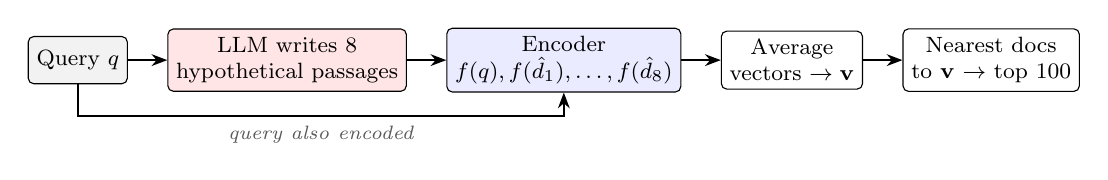
\begin{tikzpicture}[node distance=5mm]
\node[doc] (q) {Query $q$};
\node[llm, right=of q] (g) {LLM writes 8\\hypothetical passages};
\node[model, right=of g] (e) {Encoder\\$f(q),f(\hat d_1),\dots,f(\hat d_8)$};
\node[box, right=of e] (m) {Average\\vectors $\to \mathbf v$};
\node[box, right=of m] (s) {Nearest docs\\to $\mathbf v$ $\to$ top 100};
\draw[arr] (q)--(g); \draw[arr] (g)--(e); \draw[arr] (e)--(m); \draw[arr] (m)--(s);
\draw[arr] (q.south) -- ++(0,-4mm) -| node[lab, pos=0.25, below]{query also encoded} (e.south);
\end{tikzpicture}\end{center}

\paragraph{The averaged vector.} The search vector is the mean of the query embedding and the $N$
passage embeddings (the paper's Eq.~8; we use $N=8$, as the official code does):
\[
\mathbf v \;=\; \frac{1}{N+1}\Big(f(q) + \sum_{k=1}^{N} f(\hat d_k)\Big).
\]
Figure~\ref{fig:hydespace} draws this in a two-dimensional cartoon of the embedding space. Real
documents form a region (gray); the short query lands outside it. Each hypothetical passage is
written like a real document, so its vector lands \emph{inside} the document region, near the
documents that discuss the same topic. The passages differ in their invented details, so their
vectors scatter, but they share the topic, so they scatter around the same place. Averaging cancels
the sample-specific noise and keeps the shared direction; adding $f(q)$ keeps the vector anchored to
what was actually asked. Search then returns the documents with the smallest angle to $\mathbf v$.

\begin{figure}[h]\centering
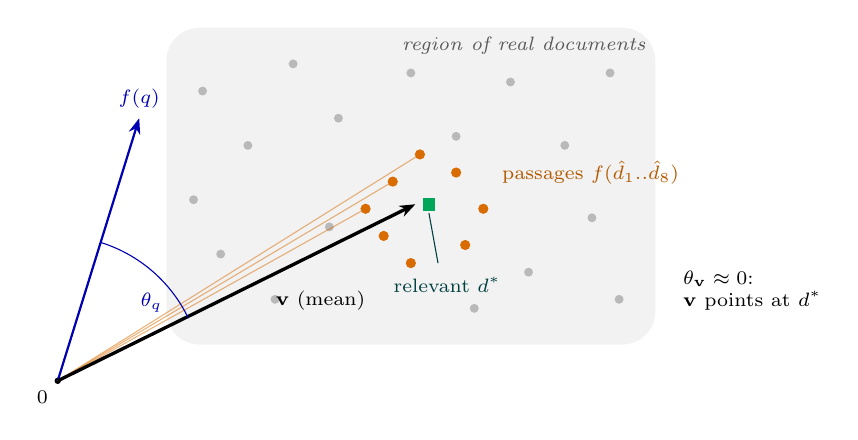
\begin{tikzpicture}[scale=1.15, >={Stealth[length=2mm]}]
  % document region and background documents
  \fill[gray!10, rounded corners=12pt] (1.2,0.4) rectangle (6.6,3.9);
  \node[lab, anchor=north east] at (6.6,3.9) {region of real documents};
  \foreach \x/\y in {1.6/3.2,2.1/2.6,2.6/3.5,3.1/2.9,3.9/3.4,4.4/2.7,5.0/3.3,5.6/2.6,6.1/3.4,
                     1.8/1.4,2.4/0.9,3.0/1.7,5.2/1.2,5.9/1.8,6.2/0.9,4.6/0.8,1.5/2.0}
    \fill[gray!55] (\x,\y) circle (1.4pt);
  % relevant document
  \fill[teal!70!green] (4.03,1.88) rectangle ++(0.14,0.14);
  \node[font=\scriptsize, teal!50!black, anchor=north] at (4.3,1.25) {relevant $d^\ast$};
  \draw[teal!50!black, thin] (4.2,1.3) -- (4.1,1.85);
  % origin and vectors
  \coordinate (O) at (0,0);
  \fill (O) circle (1pt) node[below left, font=\scriptsize]{0};
  \draw[->, thick, blue!70!black] (O) -- (0.9,2.9) node[above, font=\scriptsize]{$f(q)$};
  \foreach \x/\y in {3.7/2.2, 4.4/2.3, 3.6/1.6, 4.5/1.5, 4.0/2.5, 3.4/1.9, 4.7/1.9, 3.9/1.3}
    \fill[orange!85!black] (\x,\y) circle (1.6pt);
  \foreach \x/\y in {3.7/2.2, 4.0/2.5, 3.4/1.9}
    \draw[orange!85!black, thin, opacity=0.5] (O) -- (\x,\y);
  \node[font=\scriptsize, orange!70!black, anchor=west] at (4.8,2.3) {passages $f(\hat d_1..\hat d_8)$};
  \draw[->, very thick] (O) -- (3.95,1.95);
  \node[font=\scriptsize, anchor=north west] at (2.3,1.1) {$\mathbf v$ (mean)};
  % angle between f(q) and the relevant doc; v is almost aligned with it
  \draw[blue!70!black] (25.6:1.6) arc[start angle=25.6, end angle=72.8, radius=1.6];
  \node[font=\scriptsize, blue!70!black] at (40:1.35) {$\theta_q$};
  \node[font=\scriptsize, align=left, anchor=west] at (6.8,1.0) {$\theta_{\mathbf v}\approx 0$:\\$\mathbf v$ points at $d^\ast$};
\end{tikzpicture}
\caption{Cartoon of HyDE in embedding space. The query vector $f(q)$ points away from the document
region; the eight hypothetical passages (orange) point into it, around the relevant document. Their
mean $\mathbf v$ (black) has a much smaller angle to the relevant document ($\theta_{\mathbf v}\ll\theta_q$),
so nearest-neighbour search on $\mathbf v$ ranks it near the top. Figure~\ref{fig:hydepca} shows the
same picture for a real query.}\label{fig:hydespace}
\end{figure}

\paragraph{Why averaging works: the score is an average of similarities.} The inner product is
linear, so scoring a document against the mean vector is the same as averaging its similarity to
each of the nine vectors:
\[
\mathrm{score}(d) \;=\; \mathbf v\cdot f(d) \;=\; \frac{1}{N+1}\Big( f(q)\cdot f(d) \;+\; \sum_{k=1}^{N} f(\hat d_k)\cdot f(d)\Big).
\]
So HyDE is a vote: a document ranks high only if it is close to the query \emph{and} to most of the
passages. A document that matches one passage's invented detail gets one vote; a document on the
topic all passages share gets all of them. That is why hallucinated facts do little harm, and why
the method still needs only one nearest-neighbour search (the mean is computed once, so the cost is
the same as Dense search).
\begin{center}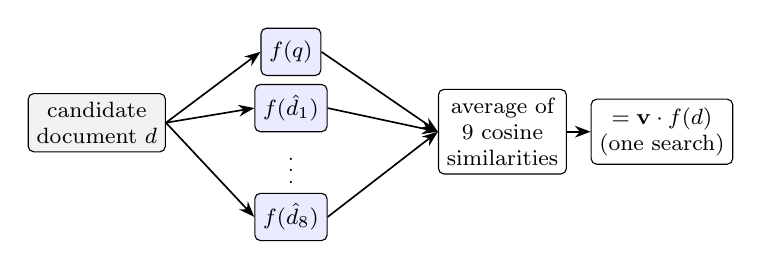
\begin{tikzpicture}[node distance=3mm]
\node[doc] (d) {candidate\\document $d$};
\node[model, right=12mm of d, yshift=9mm] (fq) {$f(q)$};
\node[model, below=1mm of fq] (h1) {$f(\hat d_1)$};
\node[below=0mm of h1, font=\scriptsize] (dots) {$\vdots$};
\node[model, below=0mm of dots] (h8) {$f(\hat d_8)$};
\foreach \n in {fq,h1,h8} \draw[arr] (d.east) -- (\n.west);
\node[box, right=14mm of h1, yshift=-3mm] (avg) {average of\\9 cosine\\similarities};
\foreach \n in {fq,h1,h8} \draw[arr] (\n.east) -- (avg.west);
\node[box, right=of avg] (eq) {$=\mathbf v\cdot f(d)$\\(one search)};
\draw[arr] (avg)--(eq);
\end{tikzpicture}\end{center}

\paragraph{Why vector length matters.} The mean treats vectors as arrows, so a longer arrow pulls
harder. bge normalizes every vector to length 1, so the query and each passage get an equal
$1/9$ say. Contriever does not normalize; its vectors grow with text length. The cartoon below
shows the effect we measured (Section~\ref{sec:hydegeo}): long LLM passages produce long vectors that
swamp $f(q)$, and the mean drifts toward whatever the passages over-emphasize.
\begin{center}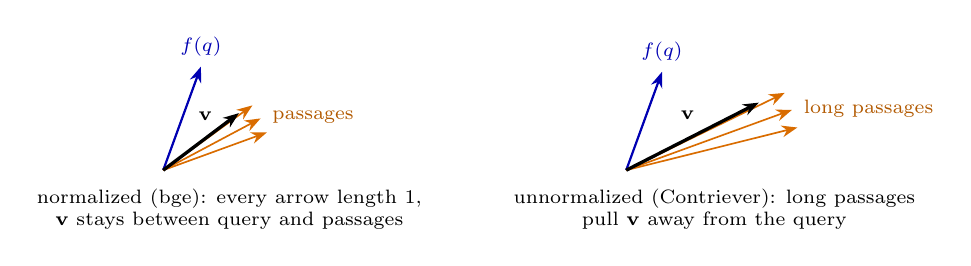
\begin{tikzpicture}[scale=1.4, >={Stealth[length=2mm]}]
  \begin{scope}
    \draw[->, thick, blue!70!black] (0,0) -- (70:1) node[above, font=\scriptsize]{$f(q)$};
    \foreach \a in {20,28,36} \draw[->, orange!85!black, semithick] (0,0) -- (\a:1);
    \draw[->, very thick] (0,0) -- (37:0.86);
    \node[font=\scriptsize] at (52:0.62) {$\mathbf v$};
    \node[font=\scriptsize, orange!70!black, anchor=west] at (28:1.02) {passages};
    \node[font=\scriptsize, align=center] at (0.6,-0.35) {normalized (bge): every arrow length 1,\\$\mathbf v$ stays between query and passages};
  \end{scope}
  \begin{scope}[xshift=4.2cm]
    \draw[->, thick, blue!70!black] (0,0) -- (70:0.95) node[above, font=\scriptsize]{$f(q)$};
    \foreach \a in {14,20,26} \draw[->, orange!85!black, semithick] (0,0) -- (\a:1.6);
    \draw[->, very thick] (0,0) -- (27:1.35);
    \node[font=\scriptsize] at (42:0.75) {$\mathbf v$};
    \node[font=\scriptsize, orange!70!black, anchor=west] at (20:1.62) {long passages};
    \node[font=\scriptsize, align=center] at (0.8,-0.35) {unnormalized (Contriever): long passages\\pull $\mathbf v$ away from the query};
  \end{scope}
\end{tikzpicture}\end{center}

\section{HyDE on real data: what the averaged vector does}\label{sec:hydegeo}
To see this mechanism in the real system, we re-encoded the cached
gpt-oss passages and measured, for every query with a judged-relevant document, how the query vector
$f(q)$, the individual passage vectors $f(\hat d_k)$ and the HyDE vector $\mathbf v$ relate to the
relevant documents. The script is \texttt{retrieval\_eval.evaluation.hyde\_geometry}; it makes no new LLM calls.
Table~\ref{tab:hydegeo} summarizes it.

\paragraph{Worked example.} SciFact (scientific claims, Section~\ref{sec:data}) claim 324 is ``Deleting Raptor reduces G-CSF levels.'' Its
relevant abstract never uses the word \emph{Raptor}; it is about ``mTOR signalling'' regulating
``G-CSF'' in mammary tumours. Searching with $f(q)$ ranks it 113th, and none of the query's top 10 is
relevant. The first gpt-oss passage begins ``Raptor, a core component of the mechanistic target of
rapamycin complex 1 (mTORC1)\ldots{} granulocyte-colony stimulating factor (G-CSF)\ldots'': it is
partly invented (it describes a mouse study that does not exist), but it supplies the missing link
\emph{Raptor}\,$\to$\,\emph{mTOR} in the vocabulary of an abstract. All eight passages do this in
slightly different words. Their mean moves the search vector into the right neighbourhood: cosine
to the relevant abstract rises from $0.646$ to $0.836$ and it is ranked \textbf{1st}.
Figure~\ref{fig:hydepca} projects this query's vectors onto their first two principal components:
the query's top-10 neighbours (blue rings) sit in the wrong area, while the eight passages cluster
next to the relevant document and the top 10 around their mean (black rings) includes it.

\begin{figure}[t]\centering
\includegraphics[width=\linewidth]{hyde_pca.pdf}
\caption{Real bge vectors for SciFact claim 324, projected to 2-D with PCA (fit on the plotted
points: 300 nearest documents to $\mathbf v$, the query's top 10 and 300 random documents). The
blue arrow is the move from $f(q)$ to the HyDE mean $\mathbf v$; thin orange lines join each
passage to the mean. A 2-D projection distorts distances, so the rings (true top 10 in 384
dimensions) are the ground truth. Chosen as the query with the largest rank gain, so it is an
illustration, not a typical case.}\label{fig:hydepca}
\end{figure}

\input{hyde_geometry.tex}

\paragraph{What the numbers show (bge).}
\begin{itemize}\itemsep 0pt
\item \textbf{The passages land in document space.} Each passage is closer to the relevant documents
than the query is (mean cosine $0.869$ vs.\ $0.773$ on SciFact, $0.718$ vs.\ $0.606$ on NFCorpus),
and the mean $\mathbf v$ is closer still ($0.879$, $0.730$): averaging removes per-sample noise.
\item \textbf{The eight passages are nearly the same vector.} Their pairwise cosine is $0.96$ on every
dataset, so the 8 samples mostly add robustness. The diversity the paper hopes for is small with
gpt-oss at temperature 0.7.
\item \textbf{Closer to everything, not only to the right thing.} $\mathbf v$ is also closer to random
documents (mean cosine $0.56\to0.65$ on SciFact), because document-like vectors share a common
direction. What matters for search is the \emph{order}, so Figure~\ref{fig:hydescatter} compares ranks.
The first relevant document moves up for 29\,\% of SciFact queries and down for 12\,\%; on NFCorpus
and FiQA the shifts are larger in both directions (31/25\,\% and 34/31\,\%); on TREC-COVID the
first relevant document is usually already at rank 1. This matches the nDCG@10 gains: large on
SciFact ($+0.056$), small on FiQA ($+0.007$).
\end{itemize}

\begin{figure}[t]\centering
\includegraphics[width=\linewidth]{hyde_scatter.pdf}
\caption{Rank of the first relevant document with the query vector ($x$) vs.\ with the HyDE vector
($y$), bge, one dot per query (log scales, slight jitter). Points below the diagonal are queries HyDE
helps.}\label{fig:hydescatter}
\end{figure}

\paragraph{The published setup does not reproduce with gpt-oss.}\label{sec:hyde}
HyDE-Contriever reaches only $0.556$ / $0.063$ / $0.434$ (SciFact / FiQA / TREC-COVID) against the
published $0.691$ / $0.273$ / $0.593$, which is \emph{below} Contriever alone. Contriever itself
reproduces exactly, so the cause is in the generated passages. gpt-oss-120b writes long answers
(median 507 words on FiQA, many with markdown headings and tables), far longer than the paper's
passages. Contriever's mean-pooled vectors are not normalized, so these long, formatted passages
dominate the averaged query vector. Stripping markdown and cutting each passage to 100 words
(HyDE-Contriever-100w) recovers SciFact ($0.684$) and FiQA ($0.285$, above the published $0.273$) but
hurts TREC-COVID ($0.351$), so it is not a general fix, and we report it as our variant, not a
reproduction. With the normalized bge encoder the same passages work well: HyDE-bge improves on Dense
on SciFact ($+0.056$), NFCorpus ($+0.021$) and FiQA ($+0.007$) and ties on TREC-COVID ($-0.002$). HyDE
is therefore sensitive to the generator's output style in a way the paper, using one generator, did
not have to address.

\paragraph{Why Contriever fails.} The same passages hurt Contriever, and the norms explain it.
Contriever's query vectors have length $\approx1.35$, the passages $\approx2.0$ and corpus
documents $\approx1.75$. In the unnormalized mean the eight long passages dominate: $\mathbf v$
keeps only a cosine of $0.51$--$0.62$ with $f(q)$, so the question itself is largely lost. On FiQA,
where gpt-oss passages are longest (502 words) and often formatted as markdown tables, the passages
are \emph{farther} from the relevant documents than the query is ($0.344$ vs.\ $0.444$), and the
median rank of the first relevant document falls from 11 to 430. Cutting passages to 100 words
reduces their norm to $\approx1.65$, which is why HyDE-Contriever-100w recovers FiQA. HyDE thus
works when (i) the generator writes passages in the corpus's style and (ii) the encoder gives
each vector an equal say. With bge both hold, and HyDE-bge is one of the best systems we tested.


\section{Applying HyDE to CCDB Search}\label{sec:ccdb}\label{sec:hydeccdb}
We chose HyDE for CCDB Search for three reasons from this study. (i) It was the strongest single
first-stage retriever on three of the four test collections: HyDE-bge has the highest nDCG@10 of any
non-reranking system on SciFact, NFCorpus and FiQA, and beats BM25 on all four (Part~II). (ii) It
needs no training and no labelled data, which matters for a collection with no relevance
judgments. (iii) It reuses an ordinary dense index: the LLM only rewrites the query, so the
narratives are embedded once and never sent to the LLM.

\paragraph{Planned pipeline.} The narratives are embedded once with a normalized encoder and stored
in a vector index. At query time the LLM writes a few complaint-style narratives for the query, these
and the query are embedded and averaged, and the index returns the nearest complaints. Because the
LLM step takes seconds, plain dense results for $f(q)$ can be shown first and replaced when the HyDE
results arrive.
\begin{center}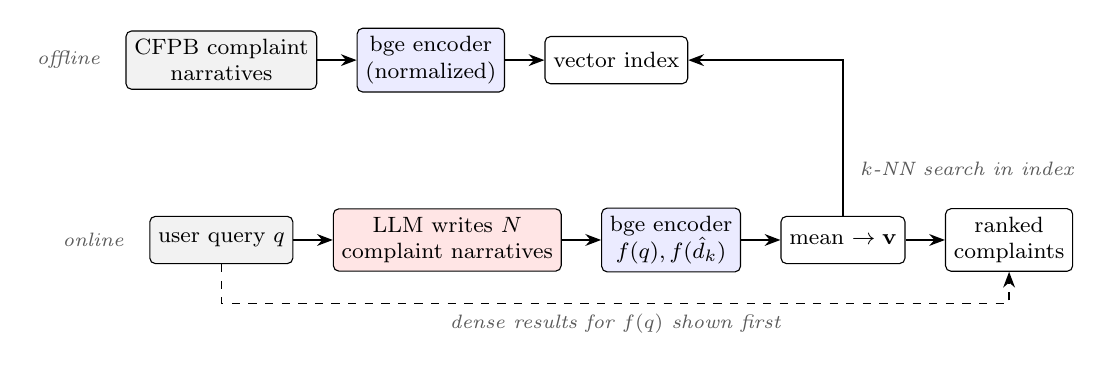
\begin{tikzpicture}[node distance=5mm]
\node[doc] (n) {CFPB complaint\\narratives};
\node[model, right=of n] (en) {bge encoder\\(normalized)};
\node[box, right=of en] (ix) {vector index};
\node[lab, left=2mm of n] {offline};
\draw[arr] (n)--(en); \draw[arr] (en)--(ix);
\node[doc, below=16mm of n] (q) {user query $q$};
\node[lab, left=2mm of q] {online};
\node[llm, right=of q] (g) {LLM writes $N$\\complaint narratives};
\node[model, right=of g] (e) {bge encoder\\$f(q), f(\hat d_k)$};
\node[box, right=of e] (v) {mean $\to\mathbf v$};
\node[box, right=of v] (r) {ranked\\complaints};
\draw[arr] (q)--(g); \draw[arr] (g)--(e); \draw[arr] (e)--(v); \draw[arr] (v)--(r);
\draw[arr] (v.north) |- (ix.east); \node[lab, anchor=west] at ($(v.north)+(1mm,6mm)$) {$k$-NN search in index};
\draw[arr, dashed] (q.south) -- ++(0,-5mm) -| node[lab, pos=0.25, below]{dense results for $f(q)$ shown first} (r.south);
\end{tikzpicture}\end{center}

\paragraph{Design choices.} The measurements of Section~\ref{sec:hydegeo} give a recipe, and a list of things that break HyDE:
\begin{itemize}\itemsep 0pt
\item \textbf{Use a normalized encoder} (bge-style, unit vectors). With Contriever's unnormalized
vectors the same passages made results \emph{worse} than no HyDE at all.
\item \textbf{Keep the query in the mean.} $f(q)$ anchors the vector to what was asked; when it was
drowned out (Contriever) relevant documents fell from rank 11 to rank 430 on FiQA.
\item \textbf{Make the prompt describe complaint narratives.} HyDE works because the passages look
like corpus documents. The paper's prompts name the document type (``scientific paper passage'',
``financial article''); for the CCDB the prompt should ask for a consumer complaint narrative, e.g.\
``Please write a consumer complaint to the CFPB describing this problem'', in plain first-person
prose of typical narrative length. gpt-oss's default style here (400--500-word markdown with headings
and tables) is far from how consumers write, and on Contriever that mismatch cost most of the gain.
\item \textbf{FiQA is the closest test, and the gain there was small.} FiQA (financial questions
answered from forum posts) is the nearest of our collections to the CCDB. HyDE-bge improved on Dense
there by only $+0.007$ nDCG@10, and 31\,\% of queries got worse. The financial domain alone does not
guarantee a large benefit; matching the narrative style (previous point) is likely what matters.
\item \textbf{Try fewer samples.} The eight passages were nearly the same vector (cosine 0.96), so
2--4 samples may give most of the benefit at lower cost. This should be tested on CCDB queries.
\item \textbf{Plan for latency.} HyDE took 10--19\,s per query here (the slowest of 8 parallel LLM
calls), against about 10\,ms for Dense. For an interactive search this needs a faster or smaller
generator, streaming, caching of frequent queries, or a fallback that shows Dense results first.
\item \textbf{Expect some queries to get worse.} 10--31\,\% of queries ranked their first relevant
document lower with HyDE. Fusing HyDE with BM25 or Dense (as Hybrid does) is a cheap hedge.
\item \textbf{Evaluate on the CCDB itself.} Gains ranged from $+0.056$ (SciFact) to $-0.002$
(TREC-COVID), so a small set of judged CCDB queries (e.g.\ labelled with the LLM judge of Section~\ref{sec:holes}, after checking it against a few human labels) is needed before relying on it.
\end{itemize}

\part{Comparison with other semantic search methods}

\section{Test collections}\label{sec:data}
The CFPB Consumer Complaint Database has no relevance judgments, so the comparison uses four
public BEIR~\cite{thakur2021beir} test collections where, as in complaint search, the query and the
relevant text tend to be worded differently (Table~\ref{tab:data}). FiQA, natural-language finance
questions answered from forum posts, is the closest to the CCDB.

\begin{table}[H]\centering\small
\caption{Collections (BEIR test splits). All queries have at least one relevant document.}\label{tab:data}
\begin{tabularx}{\linewidth}{lrrrlX}\toprule
Collection & Docs & Queries & Qrels & Grades & What it tests\\\midrule
SciFact~\cite{wadden2020scifact} & 5,183 & 300 & 339 & 1 & Scientific claims $\to$ supporting abstracts\\
NFCorpus~\cite{boteva2016nfcorpus} & 3,633 & 323 & 12,334 & 1--2 & Lay health queries $\to$ medical papers\\
FiQA-2018~\cite{maia2018fiqa} & 57,638 & 648 & 1,706 & 1 & Natural-language finance questions $\to$ forum answers\\
TREC-COVID~\cite{voorhees2020treccovid} & 171,332 & 50 & 66,336 & 0--2 & COVID questions $\to$ CORD-19 abstracts; deep pools\\
\bottomrule\end{tabularx}
\end{table}

% How each method works: one short definition and one diagram per method family.
\tikzset{
  box/.style={draw, rounded corners=2pt, align=center, font=\footnotesize, minimum height=6mm, inner sep=3pt, fill=white},
  doc/.style={box, fill=gray!10},
  llm/.style={box, fill=red!10},
  model/.style={box, fill=blue!8},
  arr/.style={-{Stealth[length=2mm]}, semithick},
  lab/.style={font=\scriptsize\itshape, text=black!65}
}

\section{How each method works}\label{sec:methods}
This section defines each method in a few sentences and shows its data flow. $q$ is the query, $d$
a document, and every method ends with a ranked list of document ids.

\subsection{BM25 (lexical baseline)~\cite{kamphuis2020bm25,thakur2021beir}}
BM25 scores a document by the query terms it contains. Each matching term contributes its inverse
document frequency (rare terms count more), damped by term frequency (controlled by $k_1$) and
normalized by document length (controlled by $b$):
$\mathrm{score}(q,d)=\sum_{t\in q}\mathrm{idf}(t)\,\frac{tf_{t,d}(k_1+1)}{tf_{t,d}+k_1(1-b+b\,|d|/\overline{|d|})}$.
Text is tokenized and stemmed first, so ``running'' matches ``run'', but ``car'' never matches
``automobile''. An inverted index makes this very fast. BM25-BEIR is the same formula with BEIR's
parameters and with title and body scored separately and summed.
\begin{center}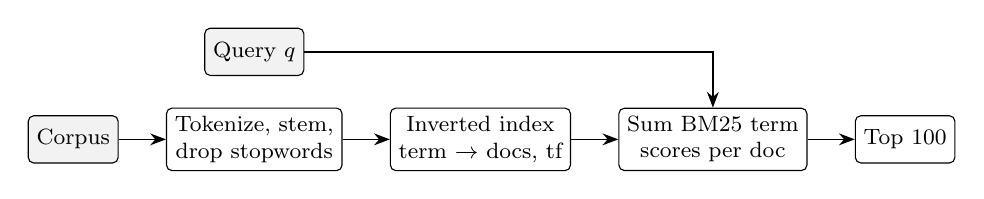
\begin{tikzpicture}[node distance=6mm]
\node[doc] (c) {Corpus};
\node[box, right=of c] (t) {Tokenize, stem,\\drop stopwords};
\node[box, right=of t] (i) {Inverted index\\term $\to$ docs, tf};
\node[box, right=of i] (s) {Sum BM25 term\\scores per doc};
\node[box, right=of s] (r) {Top 100};
\node[doc, above=4mm of t] (q) {Query $q$};
\draw[arr] (c)--(t); \draw[arr] (t)--(i); \draw[arr] (i)--(s); \draw[arr] (s)--(r);
\draw[arr] (q) -| (s);
\end{tikzpicture}\end{center}

\subsection{SPLADE (learned sparse retrieval)~\cite{formal2021splade,formal2021spladev2}}
SPLADE keeps BM25's ``bag of weighted terms'' form but lets a BERT model choose the terms and
weights. For every token position, the masked-language-model head predicts a score for each of
the 30,522 vocabulary terms. These are passed through $\log(1+\mathrm{ReLU}(\cdot))$ and max-pooled
over positions, giving one sparse vector per text. The vector also contains related terms that
never appear in the text (\emph{expansion}, e.g.\ ``car'' $\to$ ``vehicle''). Relevance is the dot
product of the query and document vectors, which an inverted index can compute.
\begin{center}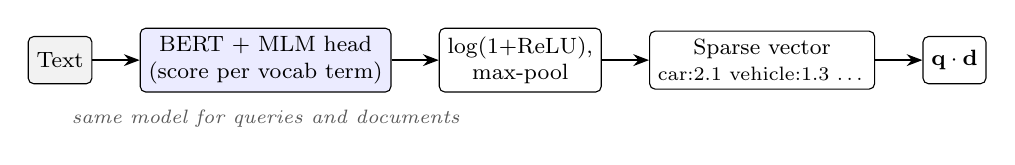
\begin{tikzpicture}[node distance=6mm]
\node[doc] (d) {Text};
\node[model, right=of d] (b) {BERT + MLM head\\(score per vocab term)};
\node[box, right=of b] (p) {$\log(1{+}\mathrm{ReLU})$,\\max-pool};
\node[box, right=of p] (v) {Sparse vector\\\scriptsize car:2.1 vehicle:1.3 \dots};
\node[box, right=of v] (s) {$\mathbf{q}\cdot\mathbf{d}$};
\draw[arr] (d)--(b); \draw[arr] (b)--(p); \draw[arr] (p)--(v); \draw[arr] (v)--(s);
\node[lab, below=1mm of b] {same model for queries and documents};
\end{tikzpicture}\end{center}

\subsection{Dense bi-encoder (Dense = bge-small, Contriever)~\cite{karpukhin2020dpr,xiao2023cpack,izacard2022contriever}}
A transformer encodes the query and each document \emph{separately} into a single dense vector
(384 dimensions for bge-small, 768 for Contriever). Training places texts with the same meaning
close together, so a query and a relevant document match even if they share no words. Relevance is
cosine similarity (bge, normalized vectors) or a dot product (Contriever). Document vectors are
computed once, offline; at query time only the query is encoded, followed by a nearest-neighbour
search. bge-small is fine-tuned on large supervised relevance data; Contriever is trained without
labels (contrastive learning on text crops), which explains its weaker results.
\begin{center}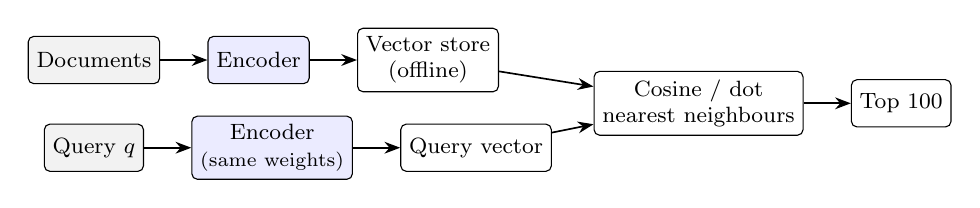
\begin{tikzpicture}[node distance=6mm]
\node[doc] (d) {Documents};
\node[model, right=of d] (ed) {Encoder};
\node[box, right=of ed] (ix) {Vector store\\(offline)};
\node[doc, below=5mm of d] (q) {Query $q$};
\node[model, right=of q] (eq) {Encoder\\\scriptsize(same weights)};
\node[box, right=of eq] (qv) {Query vector};
\node[box, right=12mm of ix, yshift=-5.5mm] (s) {Cosine / dot\\nearest neighbours};
\node[box, right=of s] (r) {Top 100};
\draw[arr] (d)--(ed); \draw[arr] (ed)--(ix); \draw[arr] (q)--(eq); \draw[arr] (eq)--(qv);
\draw[arr] (ix)--(s); \draw[arr] (qv)--(s); \draw[arr] (s)--(r);
\end{tikzpicture}\end{center}

\subsection{ColBERTv2 with PLAID (late interaction)~\cite{khattab2020colbert,santhanam2022colbertv2,santhanam2022plaid}}
ColBERT keeps one vector \emph{per token} instead of one per text. A query is scored against a
document by MaxSim: each query token finds its most similar document token, and these maxima are
summed, $\mathrm{score}=\sum_{i\in q}\max_{j\in d}\mathbf{q}_i\cdot\mathbf{d}_j$. This captures
term-level matches with contextual meaning. Storing every token vector is expensive, so ColBERTv2
compresses each one to a cluster centroid plus a 2-bit residual. PLAID first uses the centroids to
pick a small candidate set cheaply, then computes exact MaxSim only for those candidates.
\begin{center}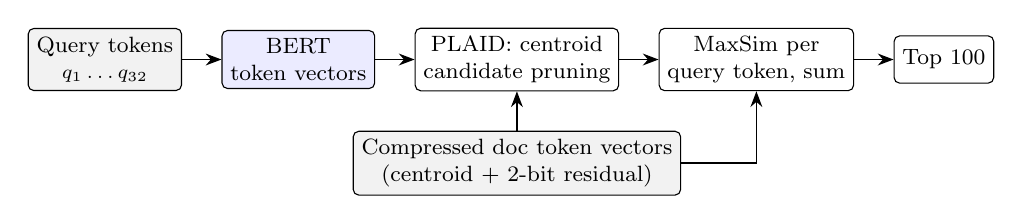
\begin{tikzpicture}[node distance=5mm]
\node[doc] (q) {Query tokens\\\scriptsize $q_1\dots q_{32}$};
\node[model, right=of q] (e) {BERT\\token vectors};
\node[box, right=of e] (c) {PLAID: centroid\\candidate pruning};
\node[box, right=of c] (m) {MaxSim per\\query token, sum};
\node[box, right=of m] (r) {Top 100};
\node[doc, below=5mm of c] (ix) {Compressed doc token vectors\\(centroid + 2-bit residual)};
\draw[arr] (q)--(e); \draw[arr] (e)--(c); \draw[arr] (c)--(m); \draw[arr] (m)--(r);
\draw[arr] (ix)--(c); \draw[arr] (ix) -| (m);
\end{tikzpicture}\end{center}

\subsection{Hybrid: Reciprocal Rank Fusion~\cite{cormack2009rrf}}
RRF merges several ranked lists using only the rank positions, so scores on different scales
(BM25 points vs.\ cosine similarities) never need calibrating. Each document receives
$\sum_{\ell}1/(60+\mathrm{rank}_\ell(d))$ over the lists that contain it. A document ranked highly
by either list, or moderately by both, rises to the top. Here the lists are the BM25 and Dense top 100.
\begin{center}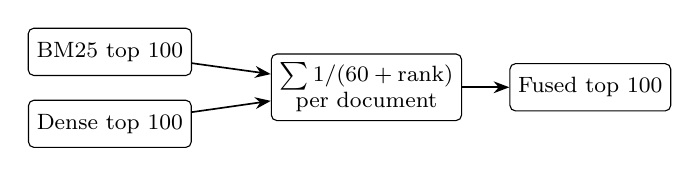
\begin{tikzpicture}[node distance=6mm]
\node[box] (b) {BM25 top 100};
\node[box, below=3mm of b] (d) {Dense top 100};
\node[box, right=10mm of b, yshift=-4.5mm] (f) {$\sum 1/(60+\mathrm{rank})$\\per document};
\node[box, right=of f] (r) {Fused top 100};
\draw[arr] (b)--(f); \draw[arr] (d)--(f); \draw[arr] (f)--(r);
\end{tikzpicture}\end{center}

\subsection{Cross-encoder reranking (Rerank, BM25+CE)~\cite{thakur2021beir,wang2020minilm}}
A cross-encoder reads the query and one document \emph{together} in a single transformer pass
(``[CLS] query [SEP] document''), so every query word can attend to every document word. It outputs
one relevance score. This is more accurate than comparing separately computed vectors, but it must
run once per (query, document) pair at query time, so it is applied only to a shortlist from a
first-stage retriever: the Hybrid top 50 (Rerank) or the BM25-BEIR top 100 (BM25+CE).
\begin{center}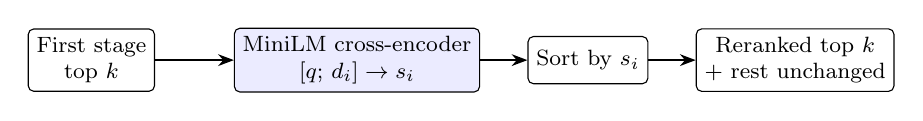
\begin{tikzpicture}[node distance=6mm]
\node[box] (f) {First stage\\top $k$};
\node[model, right=10mm of f] (ce) {MiniLM cross-encoder\\$[q;\,d_i]\to s_i$};
\node[box, right=of ce] (s) {Sort by $s_i$};
\node[box, right=of s] (r) {Reranked top $k$\\+ rest unchanged};
\draw[arr] (f)--(ce); \draw[arr] (ce)--(s); \draw[arr] (s)--(r);
\end{tikzpicture}\end{center}

\subsection{HyDE*: Hypothetical Document Embeddings~\cite{gao2023hyde}}
\paragraph{Idea.} A dense retriever compares the query vector $f(q)$ with every document vector
$f(d)$ and returns the nearest. But queries and documents are different kinds of text: a query is a
few words (``Deleting Raptor reduces G-CSF levels.''), a document is a full abstract with its own
vocabulary. Their vectors live in different parts of the space, so the nearest documents to a
\emph{query} need not be the documents that \emph{answer} it. HyDE turns retrieval into
document--document similarity, which encoders are good at: an LLM \emph{writes} $N$ plausible answer
passages $\hat d_1,\dots,\hat d_N$ (``Please write a scientific paper passage to support/refute the
claim''), and the search looks for real documents that are close to those fake ones. The passages
may contain invented facts; that does not matter, because they are never shown to the user, only
encoded. The LLM never sees the corpus.

\begin{center}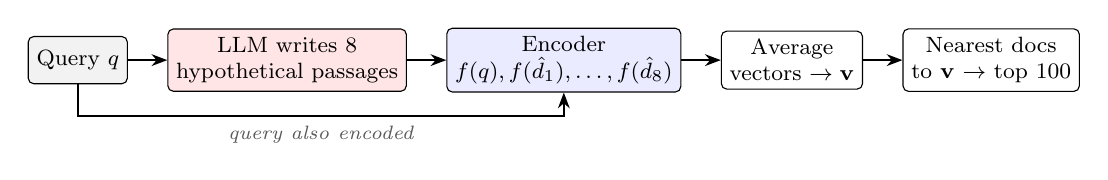
\begin{tikzpicture}[node distance=5mm]
\node[doc] (q) {Query $q$};
\node[llm, right=of q] (g) {LLM writes 8\\hypothetical passages};
\node[model, right=of g] (e) {Encoder\\$f(q),f(\hat d_1),\dots,f(\hat d_8)$};
\node[box, right=of e] (m) {Average\\vectors $\to \mathbf v$};
\node[box, right=of m] (s) {Nearest docs\\to $\mathbf v$ $\to$ top 100};
\draw[arr] (q)--(g); \draw[arr] (g)--(e); \draw[arr] (e)--(m); \draw[arr] (m)--(s);
\draw[arr] (q.south) -- ++(0,-4mm) -| node[lab, pos=0.25, below]{query also encoded} (e.south);
\end{tikzpicture}\end{center}
The search vector is the mean of $f(q)$ and the eight passage vectors, and the search itself is
the same nearest-neighbour search as Dense.

\noindent\textit{* HyDE is the method we plan to use for our project, CCDB Search (semantic search over the CFPB Consumer Complaint Database). How the averaged
vector finds the right documents, our measurements of it, and what they mean for CCDB Search are in
Section~\ref{sec:ccdb}.}

\subsection{RankGPT: listwise LLM reranking~\cite{sun2023rankgpt}}
RankGPT gives an LLM the query and 20 numbered passages and asks it to output a ranking such as
``[3] > [1] > [7] > \dots''. Because 100 passages do not fit well in one prompt, it uses a sliding
window: rerank positions 81--100, slide up by 10 to rerank 71--90, and so on to the top. Strong
documents can thus ``bubble up'' from the bottom of the list. That makes 9 LLM calls per query, which
must run in sequence. Unparseable or missing ids are appended in their original order.
\begin{center}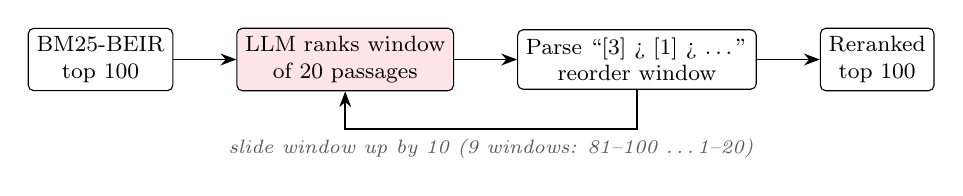
\begin{tikzpicture}[node distance=5mm]
\node[box] (b) {BM25-BEIR\\top 100};
\node[llm, right=8mm of b] (w) {LLM ranks window\\of 20 passages};
\node[box, right=8mm of w] (p) {Parse ``[3] > [1] > \dots''\\reorder window};
\node[box, right=8mm of p] (r) {Reranked\\top 100};
\draw[arr] (b)--(w); \draw[arr] (w)--(p);
\draw[arr] (p.south) -- ++(0,-5mm) -| node[lab, pos=0.25, below]{slide window up by 10 (9 windows: 81--100 \dots 1--20)} (w.south);
\draw[arr] (p)--(r);
\end{tikzpicture}\end{center}

\subsection{LLM relevance judge (evaluation aid, not a retriever)}
Human relevance labels exist only for documents that were in the original judgment pool, and
unjudged documents count as non-relevant. Following Thomas et al.~\cite{thomas2024llmjudge}, an LLM (Qwen3.5) is shown the
query and one document and asked for a 0--2 relevance grade, after considering intent match (M) and
trustworthiness (T). We first measure its agreement with human labels, then use it only to label
the unjudged documents in each system's top 10. Human labels are never overwritten.
\begin{center}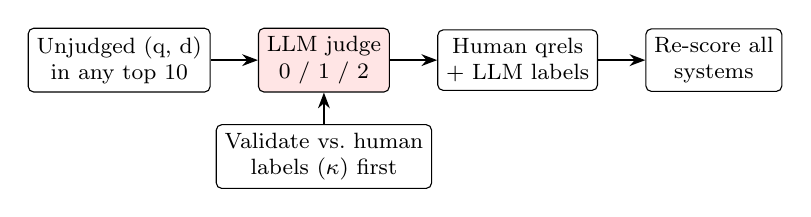
\begin{tikzpicture}[node distance=6mm]
\node[box] (u) {Unjudged (q, d)\\in any top 10};
\node[llm, right=of u] (j) {LLM judge\\0 / 1 / 2};
\node[box, right=of j] (a) {Human qrels\\+ LLM labels};
\node[box, right=of a] (e) {Re-score all\\systems};
\node[box, below=4mm of j] (v) {Validate vs.\ human\\labels ($\kappa$) first};
\draw[arr] (u)--(j); \draw[arr] (j)--(a); \draw[arr] (a)--(e); \draw[arr] (v)--(j);
\end{tikzpicture}\end{center}


\section{Systems and evaluation}
There is one script per method; all see the same corpus (title + body) and the test queries, and
each returns a top-100 list. Nothing was tuned on the test queries. Section~\ref{sec:methods} explains how each method works; Table~\ref{tab:sys} lists the
exact configurations; ``repro.'' marks a system configured to match a published result.

\begin{table}[H]\centering\small
\caption{Systems. LLM calls go through the Databricks Unity Gateway; every call is cached on disk. *\,The method planned for CCDB Search over the CFPB Consumer Complaint Database (Section~\ref{sec:ccdb}).}\label{tab:sys}
\begin{tabularx}{\linewidth}{>{\raggedright\arraybackslash}p{2.7cm}>{\raggedright\arraybackslash}p{2.6cm}X}\toprule
System & Source & Configuration\\\midrule
BM25 (baseline) & BEIR~\cite{thakur2021beir}, \cite{kamphuis2020bm25} & \texttt{bm25s}, Lucene variant, $k_1{=}1.2$, $b{=}0.75$, stopwords, Snowball stemmer\\
BM25-BEIR (repro.) & BEIR~\cite{thakur2021beir} & Anserini setting: $k_1{=}0.9$, $b{=}0.4$, Porter stemmer, title and body indexed as separate fields with scores summed\\
SPLADE (repro.) & \cite{formal2021splade,formal2021spladev2} & \texttt{naver/splade\_v2\_distil}, 256 tokens, sparse dot product\\
Dense (repro.) & DPR~\cite{karpukhin2020dpr}; \cite{xiao2023cpack,bge2023card} & \texttt{bge-small-en-v1.5}, CLS pooling, normalized, query instruction prefix, exact cosine search\\
Contriever (repro.) & \cite{izacard2022contriever}, HyDE T2~\cite{gao2023hyde} & \texttt{facebook/contriever} (unsupervised), mean pooling, unnormalized dot product\\
ColBERTv2 (repro.) & \cite{khattab2020colbert,santhanam2022colbertv2,santhanam2022plaid} & \texttt{colbertv2.0} via PyLate, PLAID index, 2-bit residuals, doc 300 / query 32 tokens\\
Hybrid & Cormack et al.~\cite{cormack2009rrf} & RRF of BM25 and Dense, $\sum 1/(60+r)$ with $r$ from 1 as in the paper\\
Rerank & BEIR~\cite{thakur2021beir}, \cite{wang2020minilm} & \texttt{ms-marco-MiniLM-L-6-v2} rescores the Hybrid top 50\\
BM25+CE (repro.) & BEIR T2~\cite{thakur2021beir} & Same cross-encoder on the BM25-BEIR top 100\\
HyDE-bge* & HyDE~\cite{gao2023hyde} & gpt-oss-120b writes 8 passages per query (temp.\ 0.7, 512 tokens, the paper's prompts); query vector = mean of query and passage embeddings; bge encoder\\
HyDE-Contriever (repro.) & HyDE~\cite{gao2023hyde} & As above with the paper's Contriever encoder\\
HyDE-Contriever-100w & ours & As above, but passages are stripped of markdown and cut to 100 words before encoding (Section~\ref{sec:hyde})\\
RankGPT (repro.) & Sun et al.~\cite{sun2023rankgpt} & Official prompts, passages cut to 300 words, sliding window 20 / step 10 over the BM25-BEIR top 100; gpt-oss-120b, temperature 0\\
\bottomrule\end{tabularx}
\end{table}

\noindent Implementation notes from checking each paper:
\begin{itemize}
\item BEIR's BM25 baseline is Anserini/Lucene with $k_1{=}0.9$, $b{=}0.4$ and multi-field indexing.
  Our default BM25 keeps the common $k_1{=}1.2$, $b{=}0.75$; it scores slightly higher on SciFact and
  FiQA and lower on TREC-COVID, so we report both.
\item PyTerrier's \texttt{RRFusion}~\cite{macdonald2020pyterrier,pyterrierdocs} uses 0-based ranks,
  i.e.\ $1/(k+r-1)$ with 1-based $r$; we follow the original paper.
\item DPR used an unnormalized dot product, FAISS HNSW search and a linear BM25 hybrid
  ($\lambda{=}1.1$). We use cosine scoring as specified by the bge model card, exact search, and RRF.
\item SPLADE scores $0.703$ on SciFact at 512 tokens; the paper's 256-token setting gives $0.693$,
  matching the published number exactly.
\item The LLMs differ from the papers': gpt-oss-120b (reasoning effort ``low'') replaces
  text-davinci-003 (HyDE) and gpt-3.5/gpt-4 (RankGPT). The judge is Qwen3.5-122B-A10B with thinking off,
  deliberately a different model from the one doing the reranking.
\end{itemize}

\textbf{Evaluation.} \texttt{ir-measures} (pytrec\_eval) on the graded test qrels: nDCG@10
(primary), Recall@100 (secondary), P@10 and AP@100; unjudged documents count as non-relevant, as in
BEIR. R$_{cap}$@100 divides by $\min(|\mathrm{rel}|,100)$, as in BEIR Table 9. Each system is compared
with BM25 on per-query nDCG@10 with a paired $t$-test. BEIR runs no significance tests; the test is
our addition, following Smucker et al.~\cite{smucker2007significance}. Latency is the mean
wall-clock time per query on an Apple M5 Max (PyTorch MPS), model load excluded. Seeds are fixed at 0.

\section{Reproductions against published results}
Table~\ref{tab:pub} puts each reproduction next to the number its paper reports. Six of seven
methods reproduce: the largest gap is $0.013$ (BM25-BEIR on TREC-COVID), and SPLADE, bge-small and
Contriever agree to within $0.003$ on every collection. BM25-BEIR also matches BEIR's capped
Recall@100 (TREC-COVID $0.499$ vs.\ $0.498$), and the cross-encoder setup matches BEIR's BM25+CE rows
to within $0.005$. These agreements matter because they show the pipeline, data and metric code are
right, so the differences in Section~\ref{sec:res} come from the methods.

\subsection{RankGPT with gpt-oss beats the published gpt-3.5 results}
Reranking the same BM25 top 100, RankGPT with gpt-oss-120b scores $0.765$ / $0.383$ / $0.878$
(SciFact / NFCorpus / TREC-COVID), against $0.704$ / $0.356$ / $0.767$ for gpt-3.5-turbo and
$0.750$ / $0.385$ / $0.855$ for gpt-4 in the paper. The gpt-4 rows reranked gpt-3.5's top 30, not BM25's
top 100, so that comparison is not like-for-like. Our BM25-BEIR first stage is also stronger than
the paper's Pyserini BM25 on TREC-COVID ($0.669$ vs.\ $0.595$), which accounts for part of the gap.
Output problems were rare: across 11,022 windows, 12 duplicate ids, 994 missing ids (appended in
original order by the official \texttt{receive\_permutation}) and 4 empty responses.
HyDE is the exception: with gpt-oss-120b and Contriever it does not reproduce the paper, for reasons
explained in Section~\ref{sec:hyde}.

\section{Results: semantic search vs.\ the BM25 baseline}\label{sec:res}
\input{tables.tex}

\begin{figure}[H]\centering
\includegraphics[width=\linewidth]{ndcg10.pdf}
\caption{nDCG@10 per system and collection; dashed line = BM25 baseline.}\label{fig:ndcg}
\end{figure}

\paragraph{Natural-language questions gain most.} On FiQA every system built on a supervised
encoder beats BM25 with $p<0.001$: Dense $+0.150$ (313 wins, 86 losses), HyDE-bge $+0.157$, and
RankGPT $+0.176$. On TREC-COVID, Dense, Hybrid, Rerank, HyDE-bge and RankGPT gain $+0.15$ to $+0.27$;
RankGPT wins 43 of 50 queries. On SciFact (declarative claims sharing technical terms with abstracts)
and NFCorpus (short topic titles), the gains are $+0.01$ to $+0.09$, and several systems are not
significantly better than BM25.

\paragraph{Supervised training transfer matters more than architecture.} Unsupervised Contriever
never beats BM25 and collapses on TREC-COVID ($0.274$), as in the HyDE paper. SPLADE and ColBERTv2,
both trained on MS MARCO, beat BM25 on FiQA and TREC-COVID but trail the much smaller bge-small, whose
training mixture is broader. The bge release does not document its English training data at the
dataset level, so some overlap with these collections cannot be ruled out (Section~\ref{sec:threats}).

\paragraph{Hybrid is the cheap, reliable choice.} RRF of BM25 and Dense is significantly better than
BM25 with $p<0.001$ on all four collections and is within $0.10$ of the best system everywhere, at
about 10\,ms per query. Its one weakness is FiQA, where equal-weight fusion with the weak BM25 list
lowers nDCG@10 from Dense's $0.403$ to $0.366$.

\paragraph{Rerankers: the small cross-encoder helps a little, the LLM a lot.} The MS MARCO MiniLM
cross-encoder adds $+0.01$ to $+0.15$ over BM25 but at most $+0.005$ over Hybrid. RankGPT on the same
BM25 list as BM25+CE is far better on every collection ($+0.076$ on SciFact, $+0.078$ on FiQA,
$+0.116$ on TREC-COVID).

\paragraph{Recall@100.} Semantic first stages miss fewer relevant documents (Table~\ref{tab:sec}),
e.g.\ FiQA $0.553\to0.727$ (HyDE-bge) and NFCorpus $0.247\to0.333$. The rerankers cannot raise
Recall@100 above that of their first stage, which matters for retrieval-augmented generation, where
the LLM only sees what the first stage retrieved.

\subsection{Judgment holes: does pooling bias favour BM25?}\label{sec:holes}
Semantic systems retrieve many documents that were never judged; scoring them as non-relevant could
understate those systems. Following Thomas et al.~\cite{thomas2024llmjudge}, we labelled every
unjudged document in any system's top 10 with an LLM judge using the paper's prompt: 63,029 pairs
in total, 18 of which failed and stay unjudged.

\textbf{Validation first.} On 200 stratified human-judged TREC-COVID pairs, the judge agrees with
humans at Cohen's $\kappa=0.53$ (binary and 3-class linear-weighted) and 62.5\% exact agreement, which
is moderate agreement. The other qrels contain only relevant documents, so $\kappa$ is undefined there;
the judge labels 80\% (SciFact) and 91\% (FiQA) of known-relevant documents as relevant, but only 27\%
on NFCorpus, whose relevance labels come from citation links rather than direct reading. The
NFCorpus augmented numbers should therefore not be relied on.

\textbf{Results.} Table~\ref{tab:aug} rescored all systems with human labels plus LLM labels for
the holes. All scores rise, because the holes contain relevant documents, and the semantic and LLM
systems gain the most: on FiQA, BM25 rises $0.253\to0.506$ while HyDE-bge rises $0.410\to0.751$ and
RankGPT $0.429\to0.799$; on TREC-COVID, Dense's gain over BM25 grows from $+0.147$ to $+0.169$. So
pooling bias does affect these comparisons, and if anything it understates the semantic methods.
One caveat applies to the LLM methods: an LLM judge may favour documents another LLM picked, even a
different model.

\section{Cost}
Table~\ref{tab:lat} gives the latencies. BM25 answers in 0.1--1.7\,ms, Dense and Hybrid in 5--10\,ms,
SPLADE in 8--83\,ms (sparse matrix product, no inverted index), and ColBERTv2/PLAID in 160--380\,ms. The
cross-encoder adds about 80\,ms over the Hybrid top 50 and 150--250\,ms over the top 100. The LLM
methods are in another class: HyDE takes 10--19\,s per query (the slowest of 8 parallel generations)
and RankGPT 26--49\,s (9 sequential windows). These were measured with 24 concurrent gateway requests,
under which per-call latency rose about 1.6$\times$, so they overstate single-user latency but not
the order of magnitude. One-time setup also differs: on TREC-COVID, BM25 indexes in 7\,s,
bge-small encodes the corpus in 6\,min, and ColBERTv2 needs 15\,min to encode plus 75\,min to build a
2.5\,GB PLAID index. The LLM steps used 10,568 (HyDE), 11,022 (RankGPT) and 63,765 (judge) gateway
calls, roughly 110M input tokens in total.

\section{Threats to validity}\label{sec:threats}
\begin{itemize}
\item \textbf{Training overlap.} bge-small's fine-tuning mixture is not documented per dataset, so
  overlap with FiQA's or NFCorpus' training splits cannot be excluded. The ColBERTv2, SPLADE and
  Contriever results do not have this caveat.
\item \textbf{Different LLMs.} gpt-oss-120b is not the model the HyDE and RankGPT papers used, and it
  is a much newer and stronger model than gpt-3.5. The RankGPT comparison shows what the method does
  with a current open-weight model, not a replication of the paper's numbers.
\item \textbf{Lexical bias in the pools.} BEIR (Table 4) found TREC-COVID's pool still lexically
  biased despite its depth. J@10 shows our top-10 lists are mostly judged there (0.88 for both Dense
  and BM25), and filling the holes did not reverse any conclusion, but it remains a caveat.
\item \textbf{Judge quality.} $\kappa=0.53$ is moderate, and the judge disagrees with the NFCorpus
  labels. The augmented results are supporting evidence, not a replacement for the human qrels.
\item \textbf{Multiple comparisons.} We ran 48 tests against BM25. With Bonferroni ($0.05/48\approx0.001$),
  only results marked $^{**}$ survive; all conclusions above rest on those.
\item \textbf{Small query set.} TREC-COVID has only 50 queries, although its main effects have
  $p<10^{-4}$.
\item \textbf{Fixed configurations and one machine.} Each system ran one configuration, chosen before
  seeing results; latency was measured on one laptop and is indicative only.
\end{itemize}

\section{Conclusion}\label{sec:concl}
\textbf{For CCDB Search.} HyDE with a normalized encoder is a strong, training-free way to bridge the
gap between short queries and long consumer-written narratives: it was the best first-stage
retriever on three of four collections, and the geometry analysis shows why it works and when it
breaks. Its costs are latency (10--19\,s per query with 8 samples) and per-query variance (10--31\,\%
of queries rank their first relevant document lower). Both can be managed: fewer samples, a faster
generator, caching, fusion with dense or BM25 results, and showing dense results first. The prompt
should ask for complaint narratives in the consumers' own style, and the system should be checked on
a small set of judged CCDB queries before it is relied on.


\textbf{Semantic search in general.} Against BM25, semantic search helped on every collection:
\begin{itemize}
\item \textbf{SciFact:} yes, modestly for cheap methods (Hybrid $+0.045$, $p<0.001$), substantially for
  LLM methods (HyDE-bge $+0.090$, RankGPT $+0.086$).
\item \textbf{NFCorpus:} yes, modestly (Hybrid $+0.042$, RankGPT $+0.064$, both $p<0.001$).
\item \textbf{FiQA:} yes, strongly (Dense $+0.150$, RankGPT $+0.176$, $p<0.001$); fusion with the weak
  BM25 list gives back a quarter of Dense's gain.
\item \textbf{TREC-COVID:} yes, strongly (Hybrid $+0.169$, RankGPT $+0.268$, $p<0.001$).
\end{itemize}
Semantic search helps most when queries are natural-language questions worded differently from the
documents, which is the CCDB Search setting. A small supervised bi-encoder fused with BM25 delivers
most of the gain for about 10\,ms per query, and LLM reranking (RankGPT) delivers the best quality
measured here at roughly 3,000--5,000 times the latency. HyDE sits between them: better than any
other first-stage retriever on most collections, for the price of one LLM call per query.

\bibliographystyle{plainnat}
\bibliography{references}

\appendix
\section{Reproducibility}\sloppy
Run \texttt{python3 -m retrieval\_eval.data.fetch\_beir \&\& .venv/bin/python run.py}. Each method is one module in \texttt{retrieval\_eval/methods/} (e.g.\ \texttt{python -m retrieval\_eval.methods.splade}); scoring, the LLM judge and the published reference numbers are in \texttt{retrieval\_eval/evaluation/}. ColBERTv2 runs in a
separate \texttt{.venv-colbert} (PyLate pins an older torch). The LLM steps need
\texttt{databricks auth} access to the Unity Gateway; with the shipped \texttt{llm\_cache/} they make
no new calls (\texttt{--no-llm} skips them). Library versions, model revisions and probe output are in
\texttt{RESULT.md}; judge labels are in \texttt{llm\_labels/} and augmented qrels in \texttt{qrels\_aug/}.

\end{document}
